\documentclass[11pt]{article}
\usepackage[final]{graphicx}
\usepackage{subcaption}
\usepackage[utf8]{inputenc}
\usepackage{listings}
\usepackage{color}
\usepackage{fancyhdr}
\usepackage{enumerate}
\usepackage{enumitem}
\usepackage{hyperref}
\usepackage{wordlike}

% \makeatletter
% \setlength{\@fptop}{0pt}
% \makeatother

% Make hyperlinks prettier
\hypersetup{
    colorlinks=true,
    linkcolor=blue,
    filecolor=magenta,      
    urlcolor=cyan,
}

% Python code formatting
\definecolor{codegreen}{rgb}{0,0.6,0}
\definecolor{codegray}{rgb}{0.5,0.5,0.5}
\definecolor{codepurple}{rgb}{0.58,0,0.82}
\definecolor{backcolour}{rgb}{0.95,0.95,0.92}
 
\lstdefinestyle{mystyle}{
    backgroundcolor=\color{backcolour},
    commentstyle=\color{codegreen},
    keywordstyle=\color{magenta},
    numberstyle=\tiny\color{codegray},
    stringstyle=\color{codepurple},
    basicstyle=\small,
    breakatwhitespace=false,
    breaklines=true,
    captionpos=t,
    keepspaces=true,
    numbers=left,
    numbersep=5pt,
    showspaces=false,
    showstringspaces=false,
    showtabs=false,
    tabsize=2
}

\lstset{style=mystyle}

\setlist{parsep=0pt,listparindent=\parindent}

% Header settings  
\pagestyle{fancy}
\fancyhf{}
\rhead{10/06/2016}
\chead{Paul Ruess}
\lhead{CE 385S -- Homework 3}
\rfoot{Page \thepage}

\begin{document}

\section*{\centerline{Homework 3 -- Problem 4}}

This project has been improved since the previous deliverable in the following ways: 

\begin{enumerate}
  \item Using the hydraulic properties computed with the Height Above Nearest Drainage (HAND) method, I have back-calculated the average manning's $n$ for each United States Geological Survey (USGS) rating curve in the Onion Creek, TX watershed. 
  \item For each USGS gage station, I have found the first instance of flow (ie. flow of 0.01 cfs) and mapped the associated stage-height as the channel bottom-depth. 
  \item Using the back-calculated manning's $n$, I have tilted the HAND rating curve for an approximate fit to the USGS rating curve with a new bottom-depth. 
\end{enumerate}

Examples of a few rating curves, as compared to their previously "manually" optimized manning's $n$ values, are included in figures 1, 2 and 3. Note that these graphs are not strictly comparable, due to the fact that changes have been made to both the USGS curve (bottom-depth shift) and the HAND curve (different manning's $n$ used). Furthermore, it is important to be aware that an average manning's $n$ (from the various manning's $n$ values calculated from the USGS data at each 1-foot interval) was applied to the HAND rating curve, and this averaging is likely not the best approach for this application; possible improvements could be made by using a root-mean-square-error (RMSE) approach for assessing the optimal manning's $n$ with this back-calculating approach. Finally, it is important to be aware that, though these automatic adjustments seem to fit the USGS rating curves fairly well, this will not be a sustainable model for large-scale rating curve optimization as it relies entirely on USGS rating curves for determining which manning's $n$ to use for the HAND rating curve snapping. 

% \begin{equation}
% Q = \frac{k}{n}AR^\frac{2}{3}S^\frac{1}{2}
% \end{equation}
% where: 
% \begin{description}
% \item[Q] is the discharge (L\textsuperscript{3}/T; ft/s, m/s);
% \item[A] is the cross-sectional area (L\textsuperscript{2}; ft\textsuperscript{2}, m\textsuperscript{2});
% \item[R] is the hydraulic radius (L; ft, m);
% \item[S] is the channel bed slope at constant water depth (L/L, ft/ft, m/m).
% \item[k] is a conversion factor, 1.0 for SI units and 1.49 for English units.
% \end{description}

% \vspace{1ex}
% \clearpage

\begin{figure}[h]
\makebox[\linewidth][c]{
\begin{subfigure}{0.65\textwidth}
  \centering
  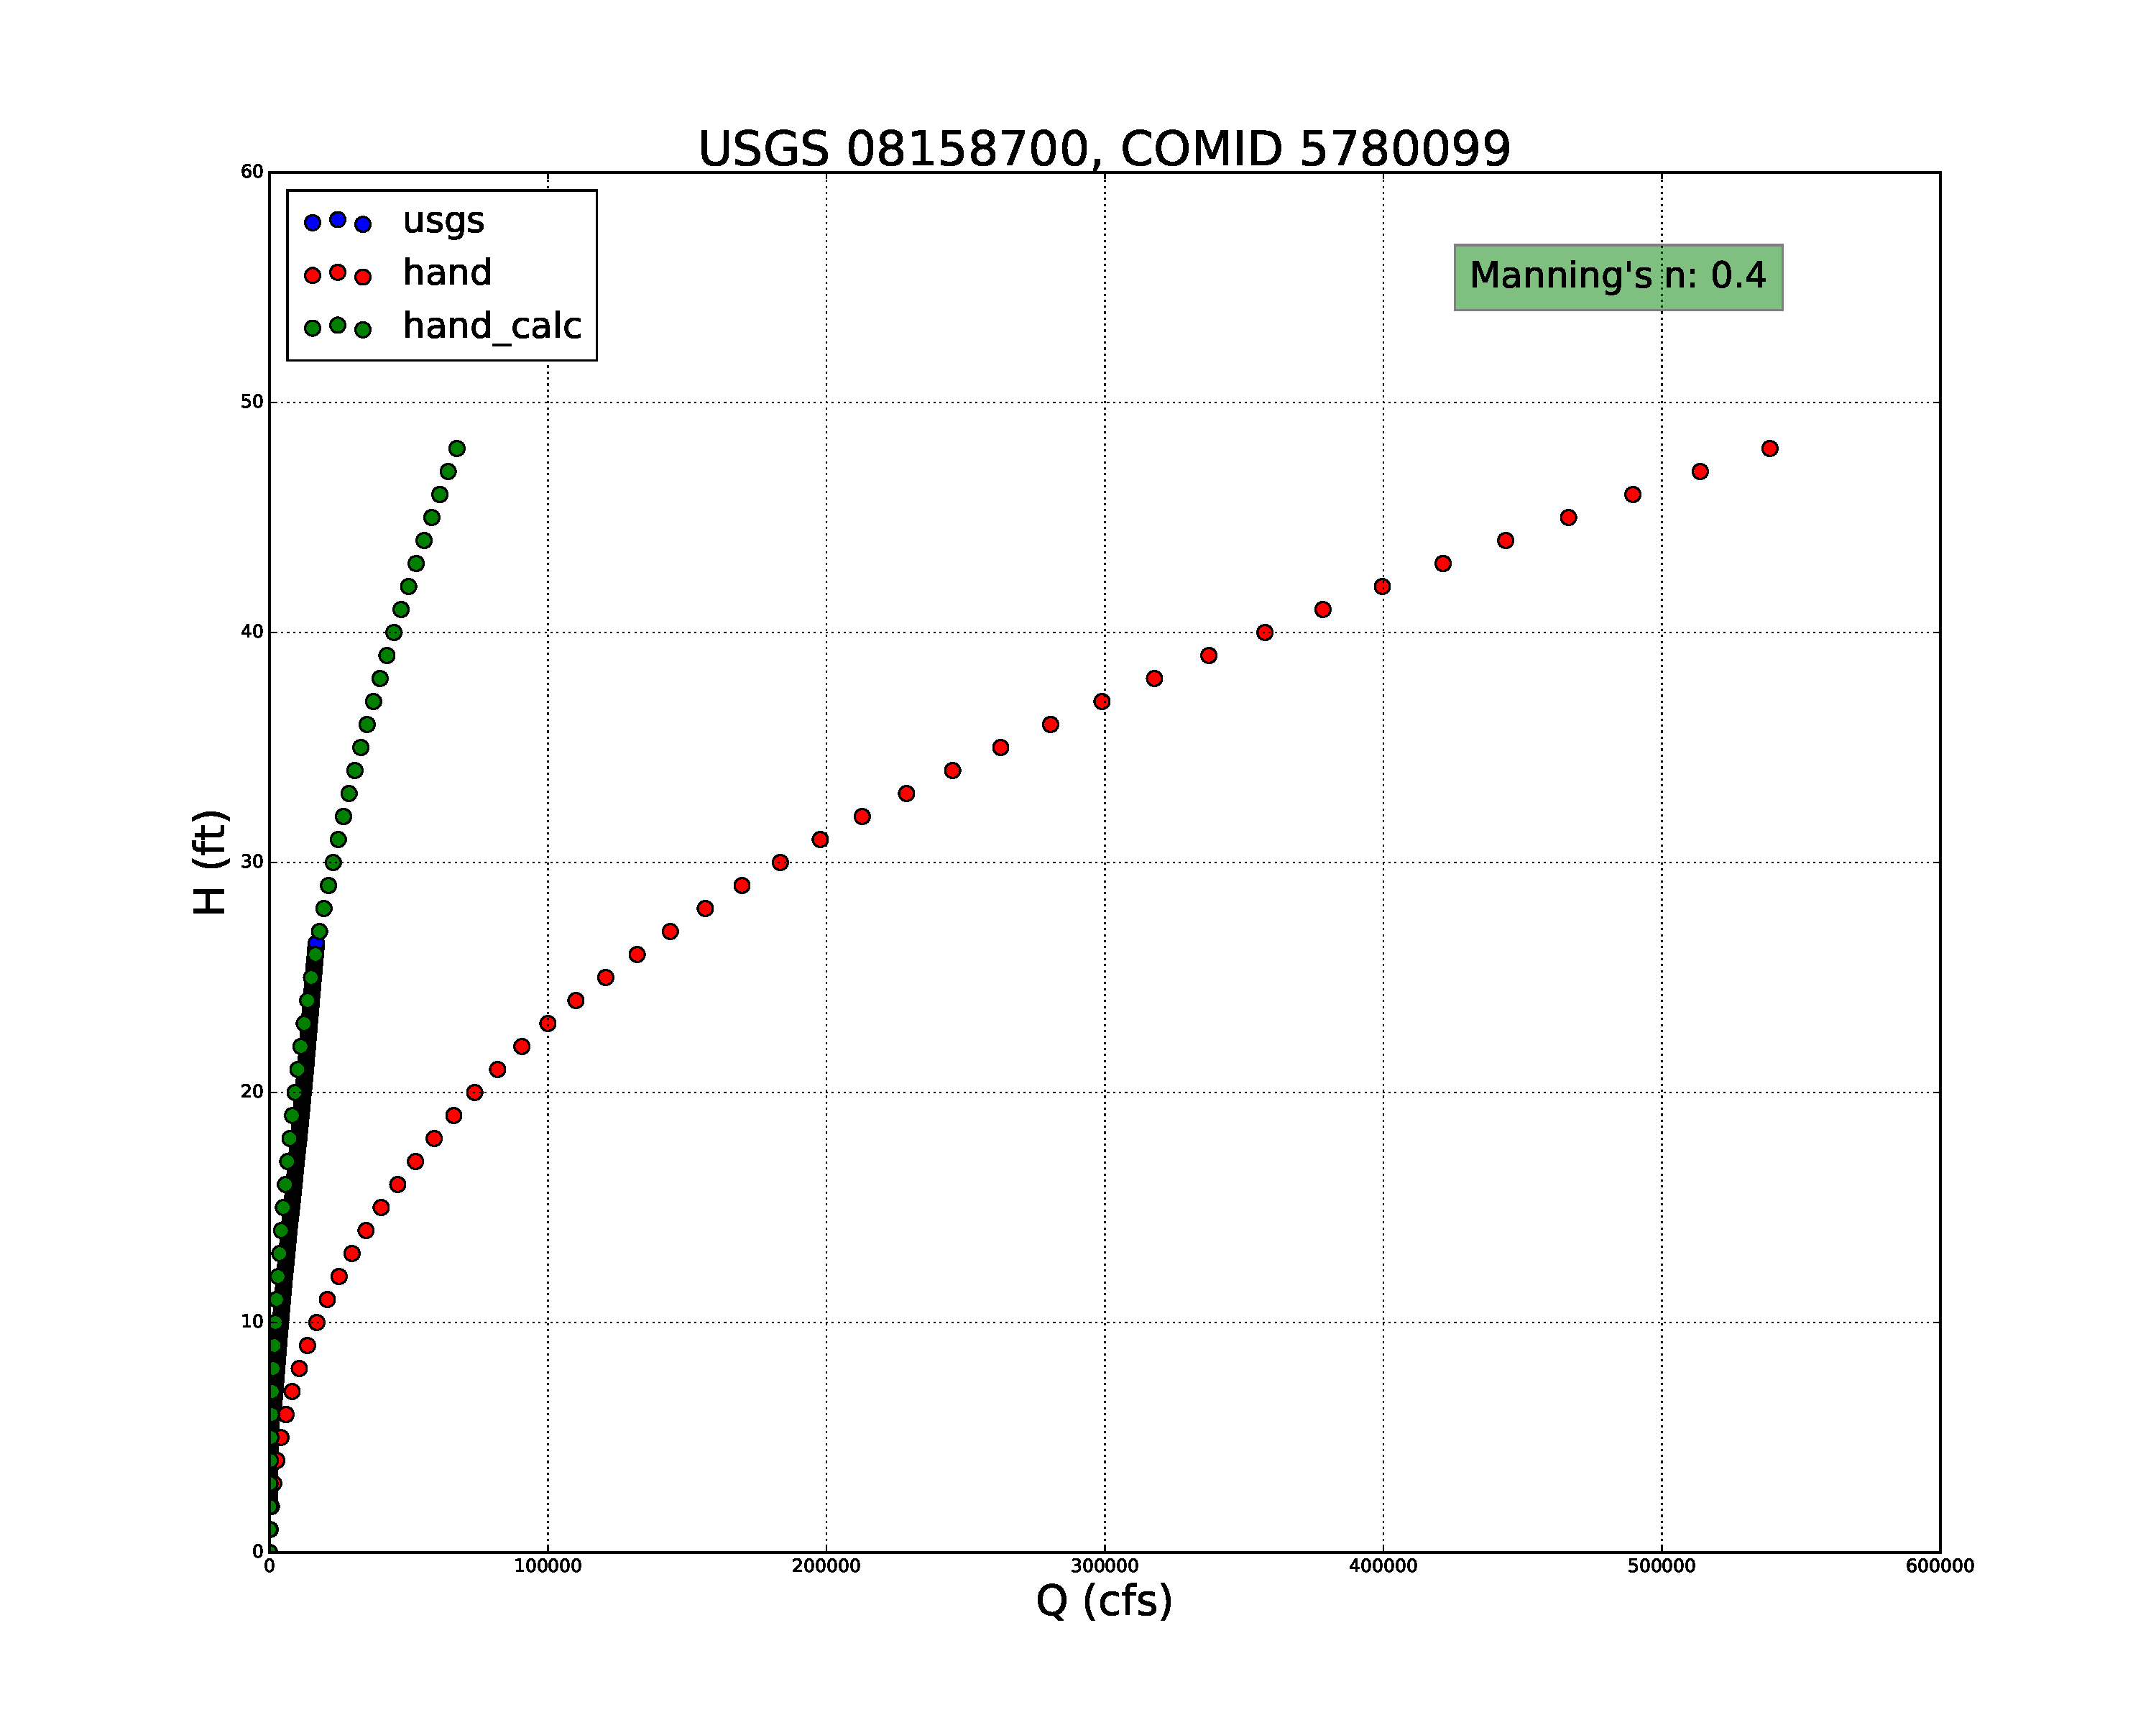
\includegraphics[width=\linewidth]{manualresults/rc_comid_5780099.pdf}
  \caption{Manually-Adjusted Rating Curve}\label{fig:a}
\end{subfigure}\hspace*{\fill}
\begin{subfigure}{0.65\textwidth}
  \centering
  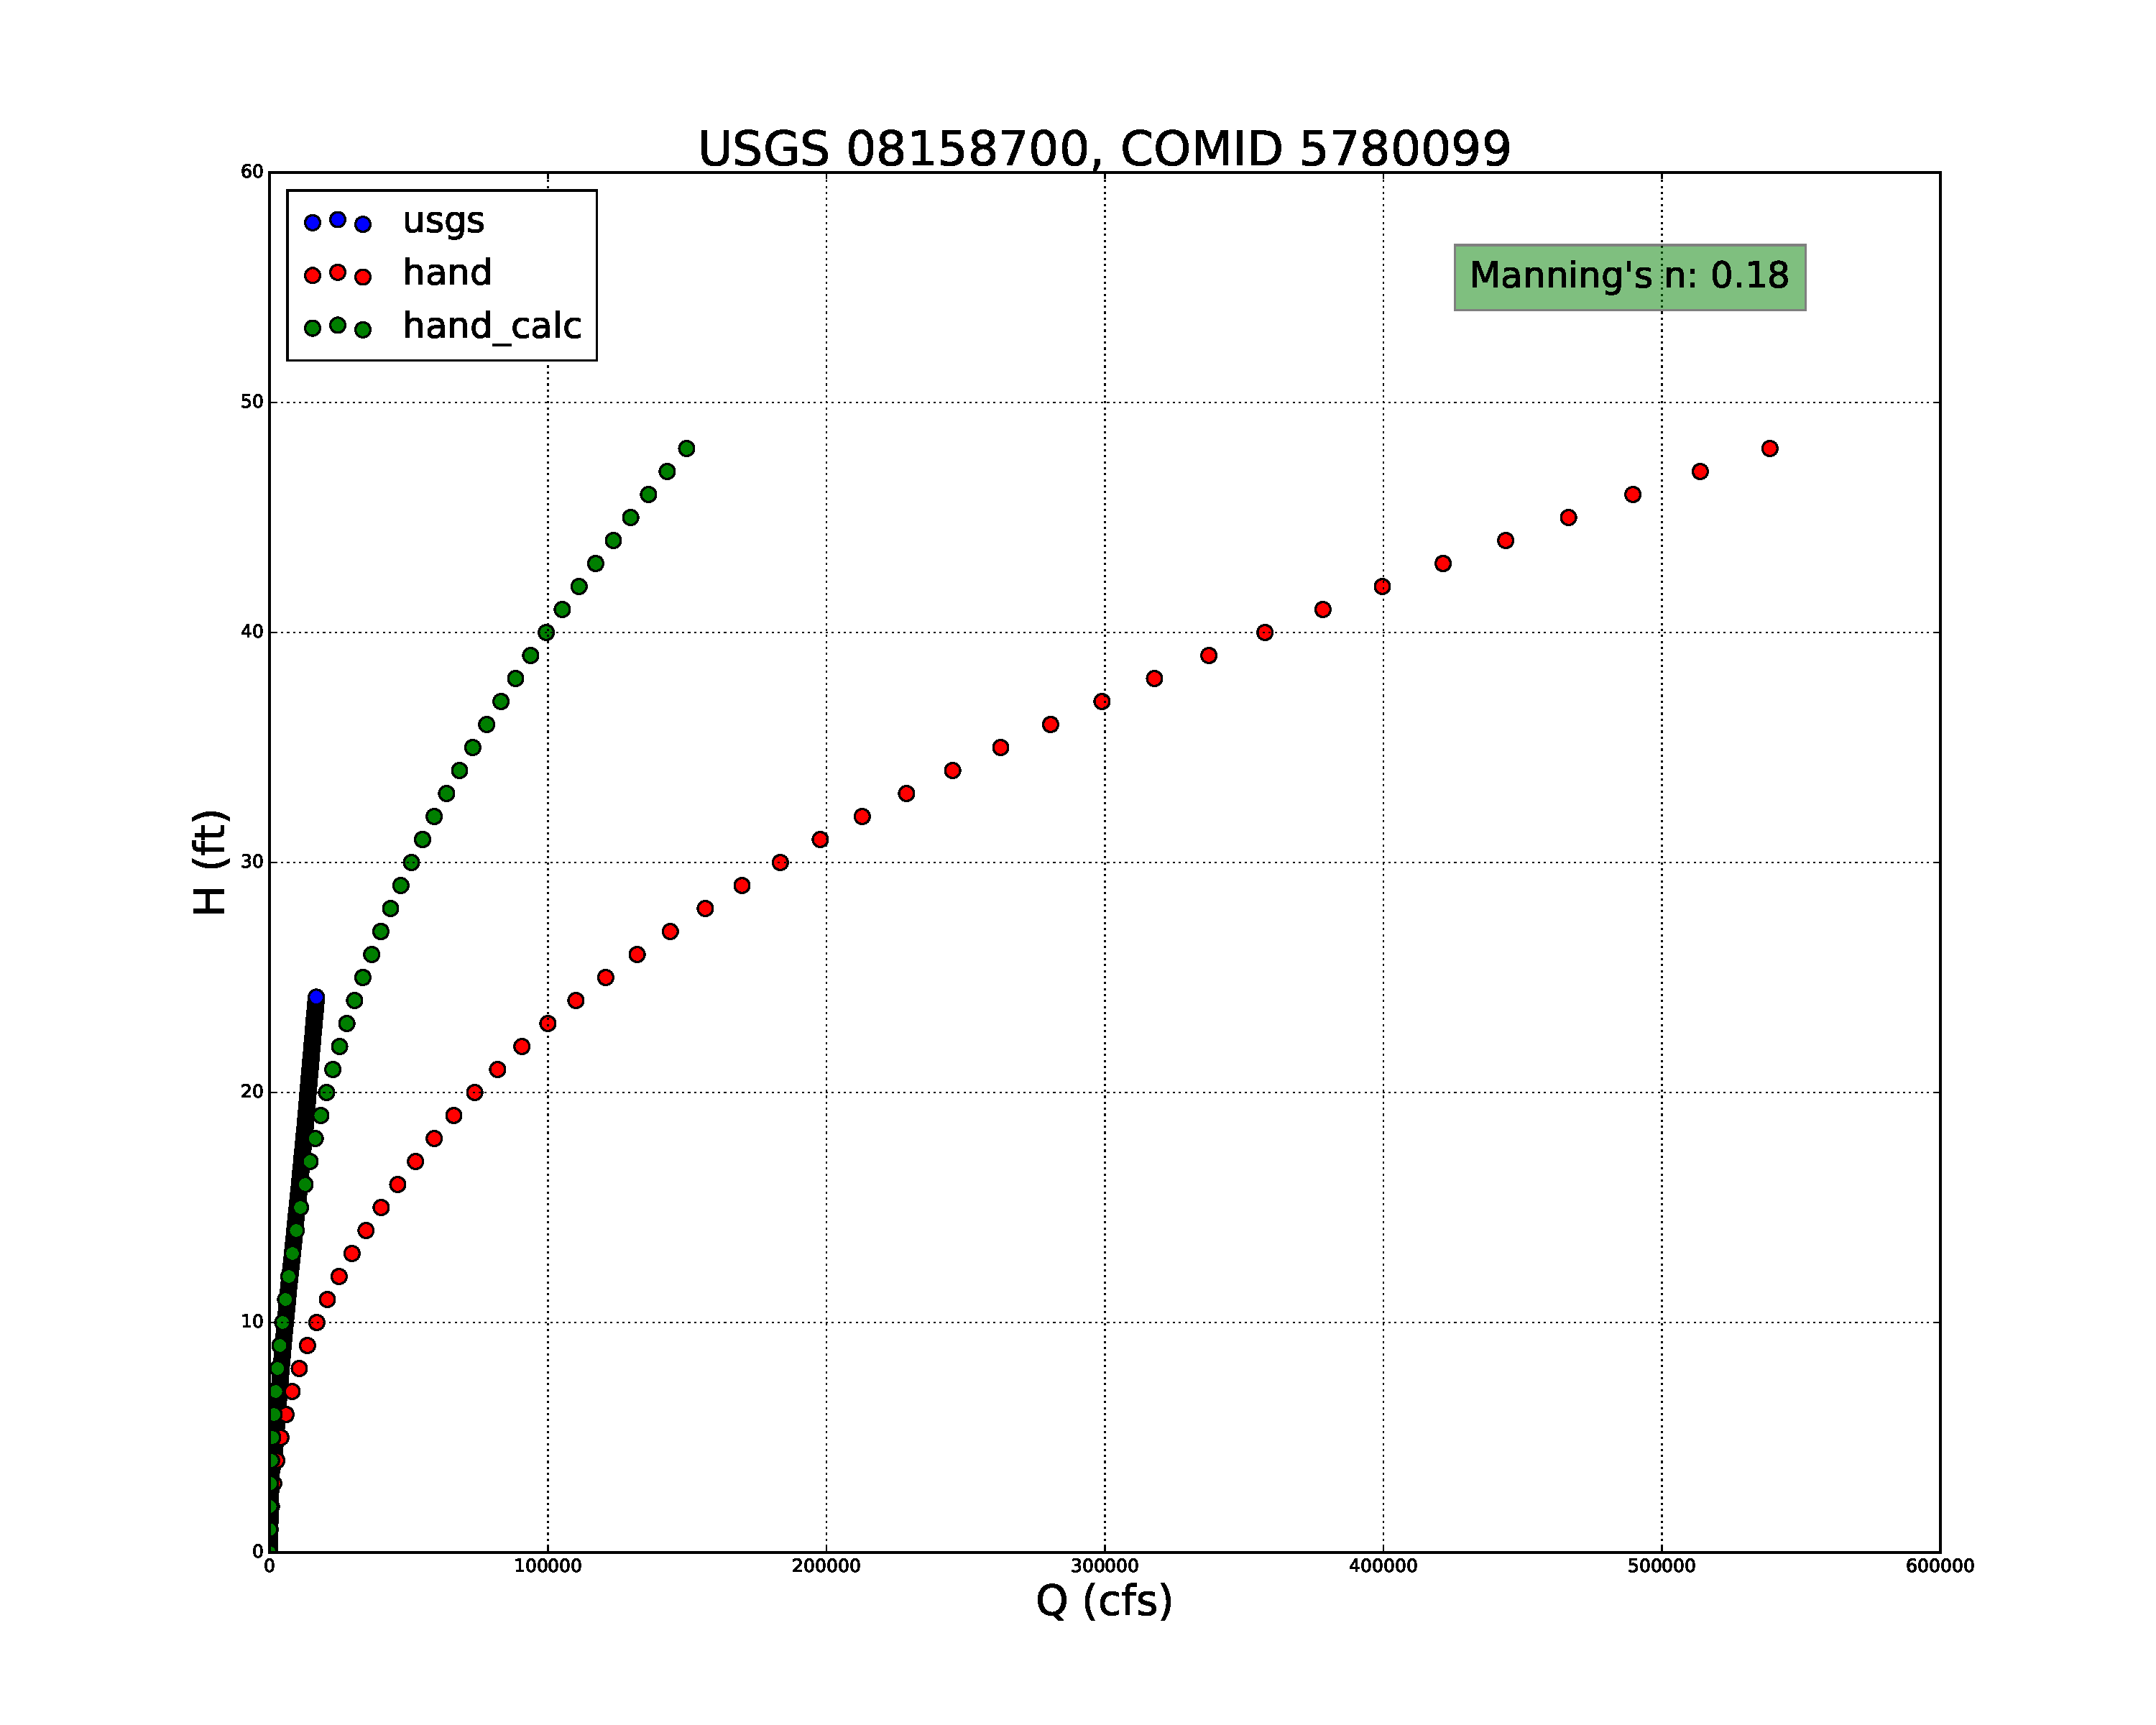
\includegraphics[width=\linewidth]{autoresults/rc_comid_5780099.pdf}
  \caption{Automatically-Adjusted Rating Curve}\label{fig:b}
\end{subfigure}\hspace*{\fill}
}
\caption{Manual vs. Automatic Adjustments for COMID 5780099 Rating Curve} \label{fig:2}
\end{figure}

\begin{figure}[h]
% \ContinuedFloat
\makebox[\linewidth][c]{
\begin{subfigure}{0.65\textwidth}
  \centering
  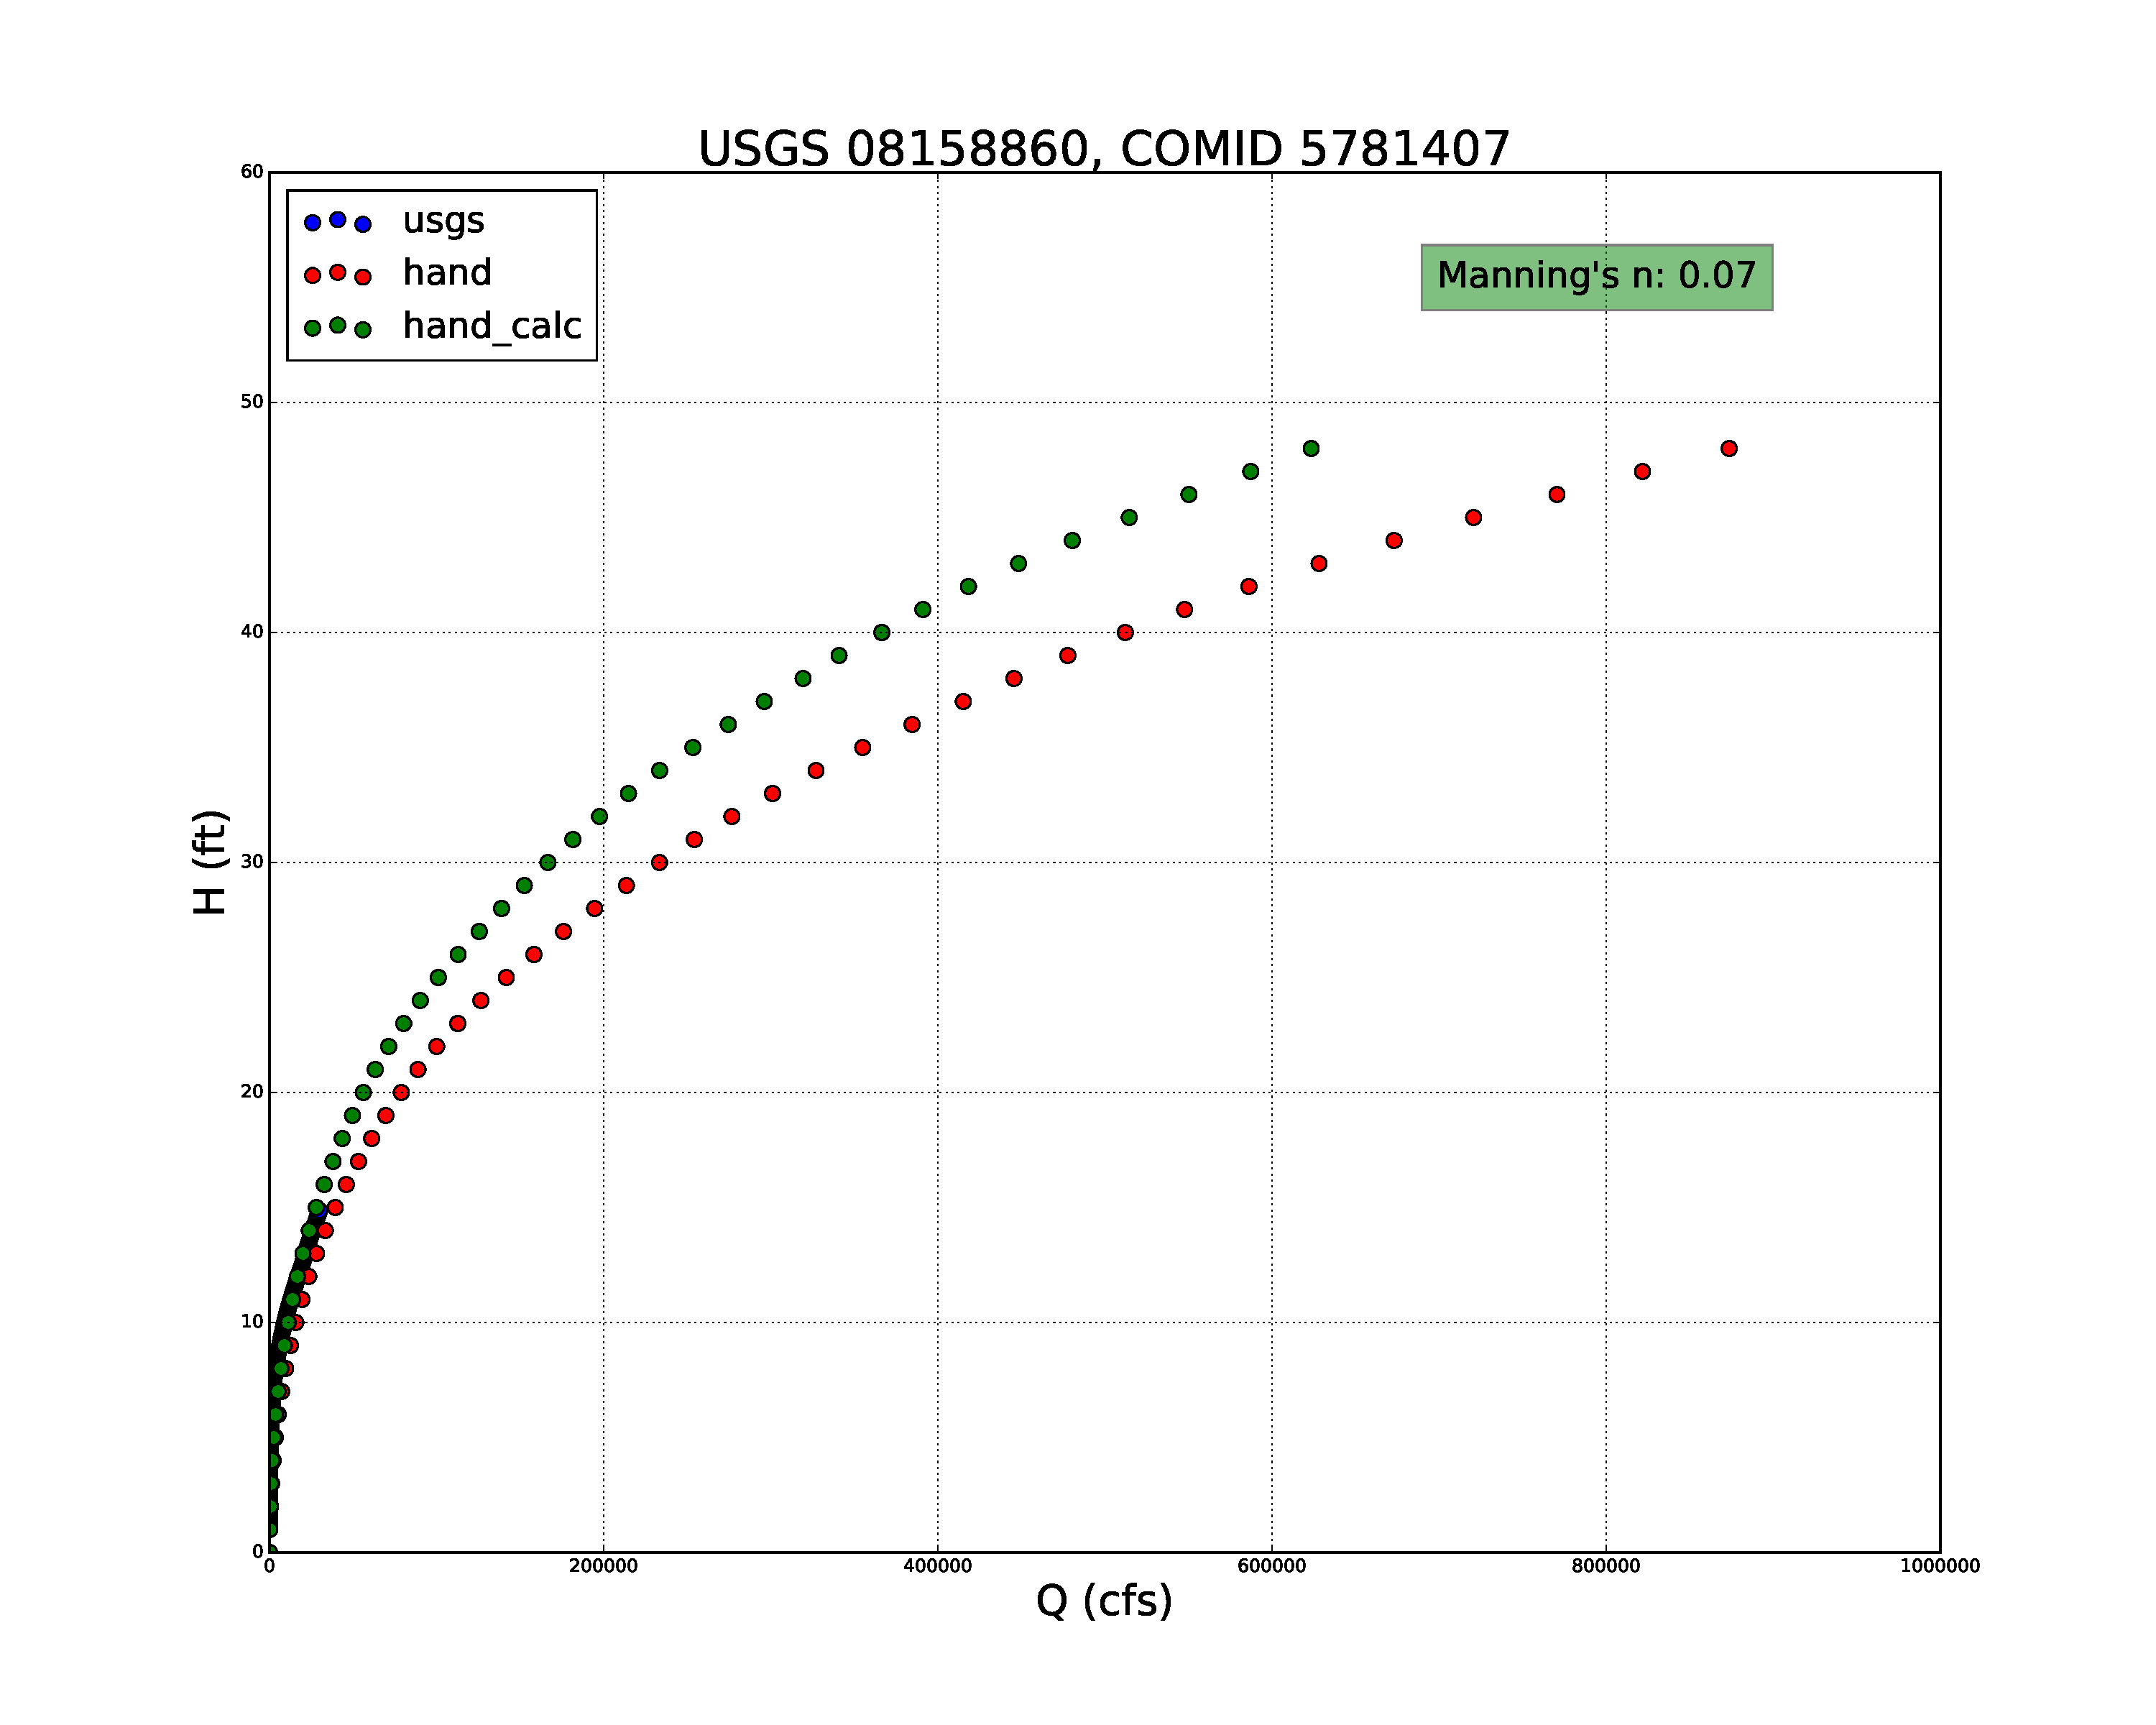
\includegraphics[width=\linewidth]{manualresults/rc_comid_5781407.pdf}
  \caption{Manually-Adjusted Rating Curve}\label{fig:a}
\end{subfigure}\hspace*{\fill}
\begin{subfigure}{0.65\textwidth}
  \centering
  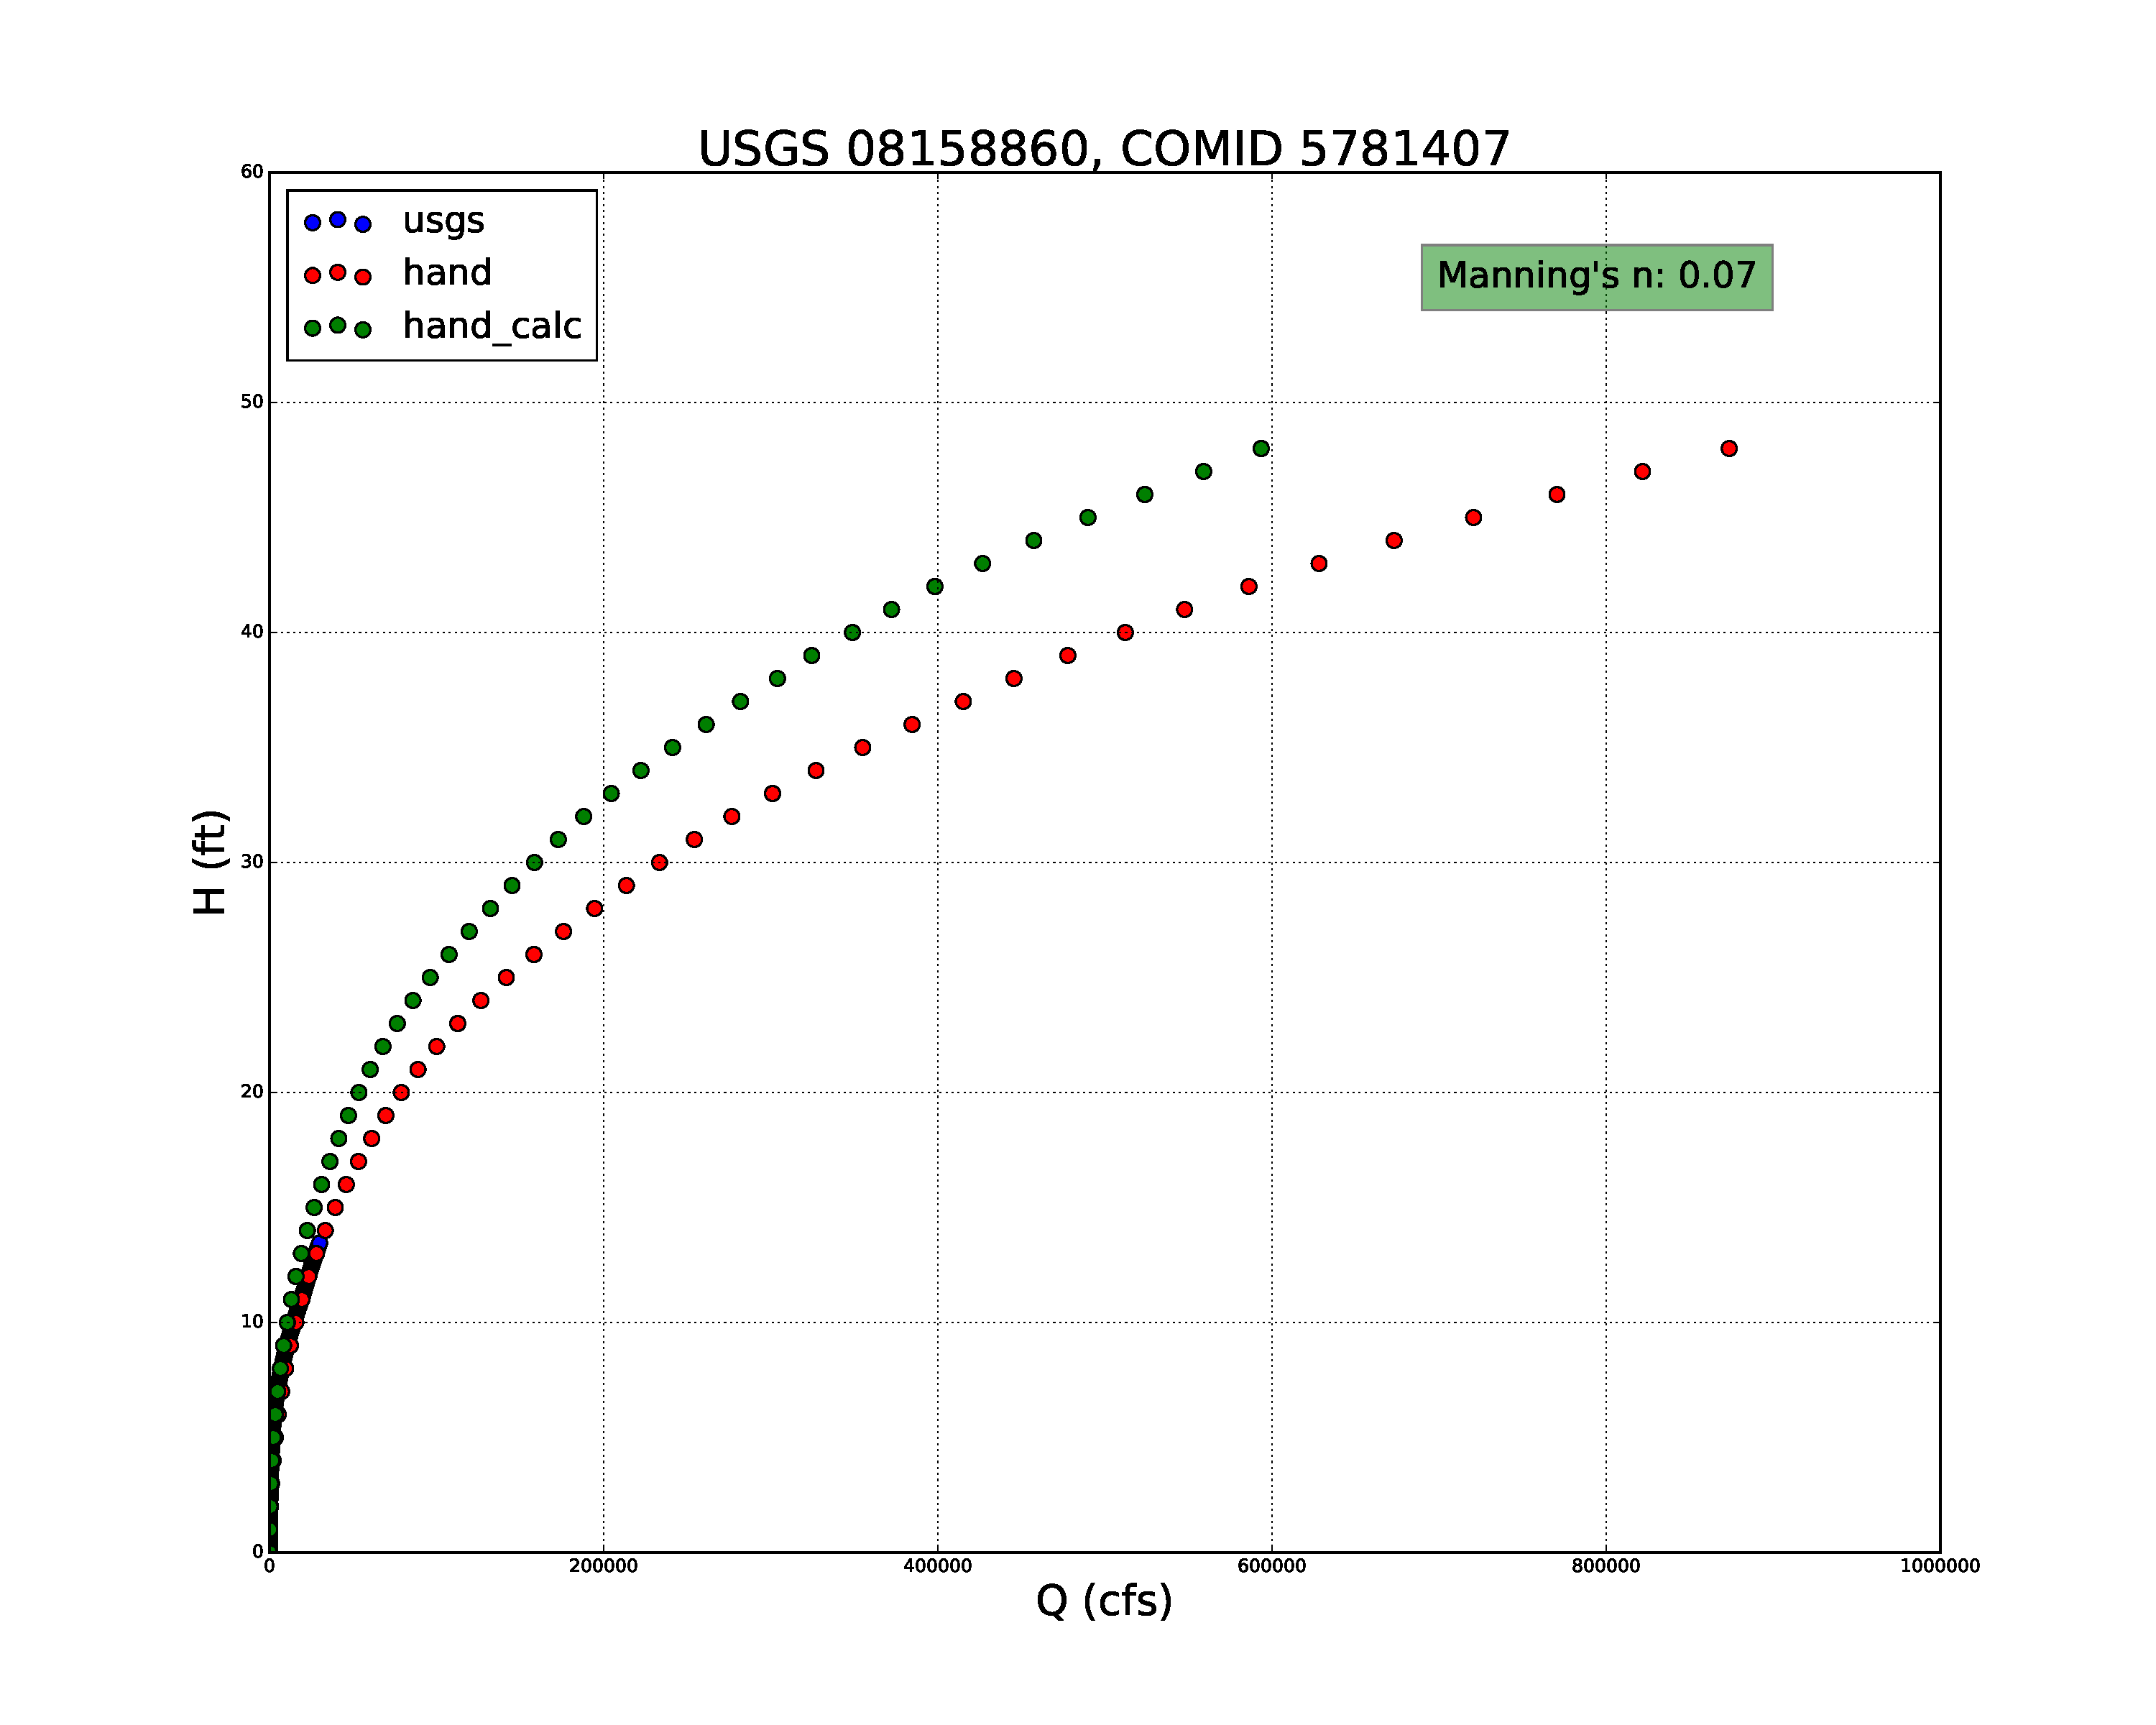
\includegraphics[width=\linewidth]{autoresults/rc_comid_5781407.pdf}
  \caption{Automatically-Adjusted Rating Curve}\label{fig:b}
\end{subfigure}\hspace*{\fill}
}

\caption{Manual vs. Automatic Adjustments for COMID 5781407 Rating Curve} \label{fig:3}
\end{figure}

\begin{figure}[h]
% \ContinuedFloat
% \smallskip
\makebox[\linewidth][c]{
\begin{subfigure}{0.65\textwidth}
  \centering
  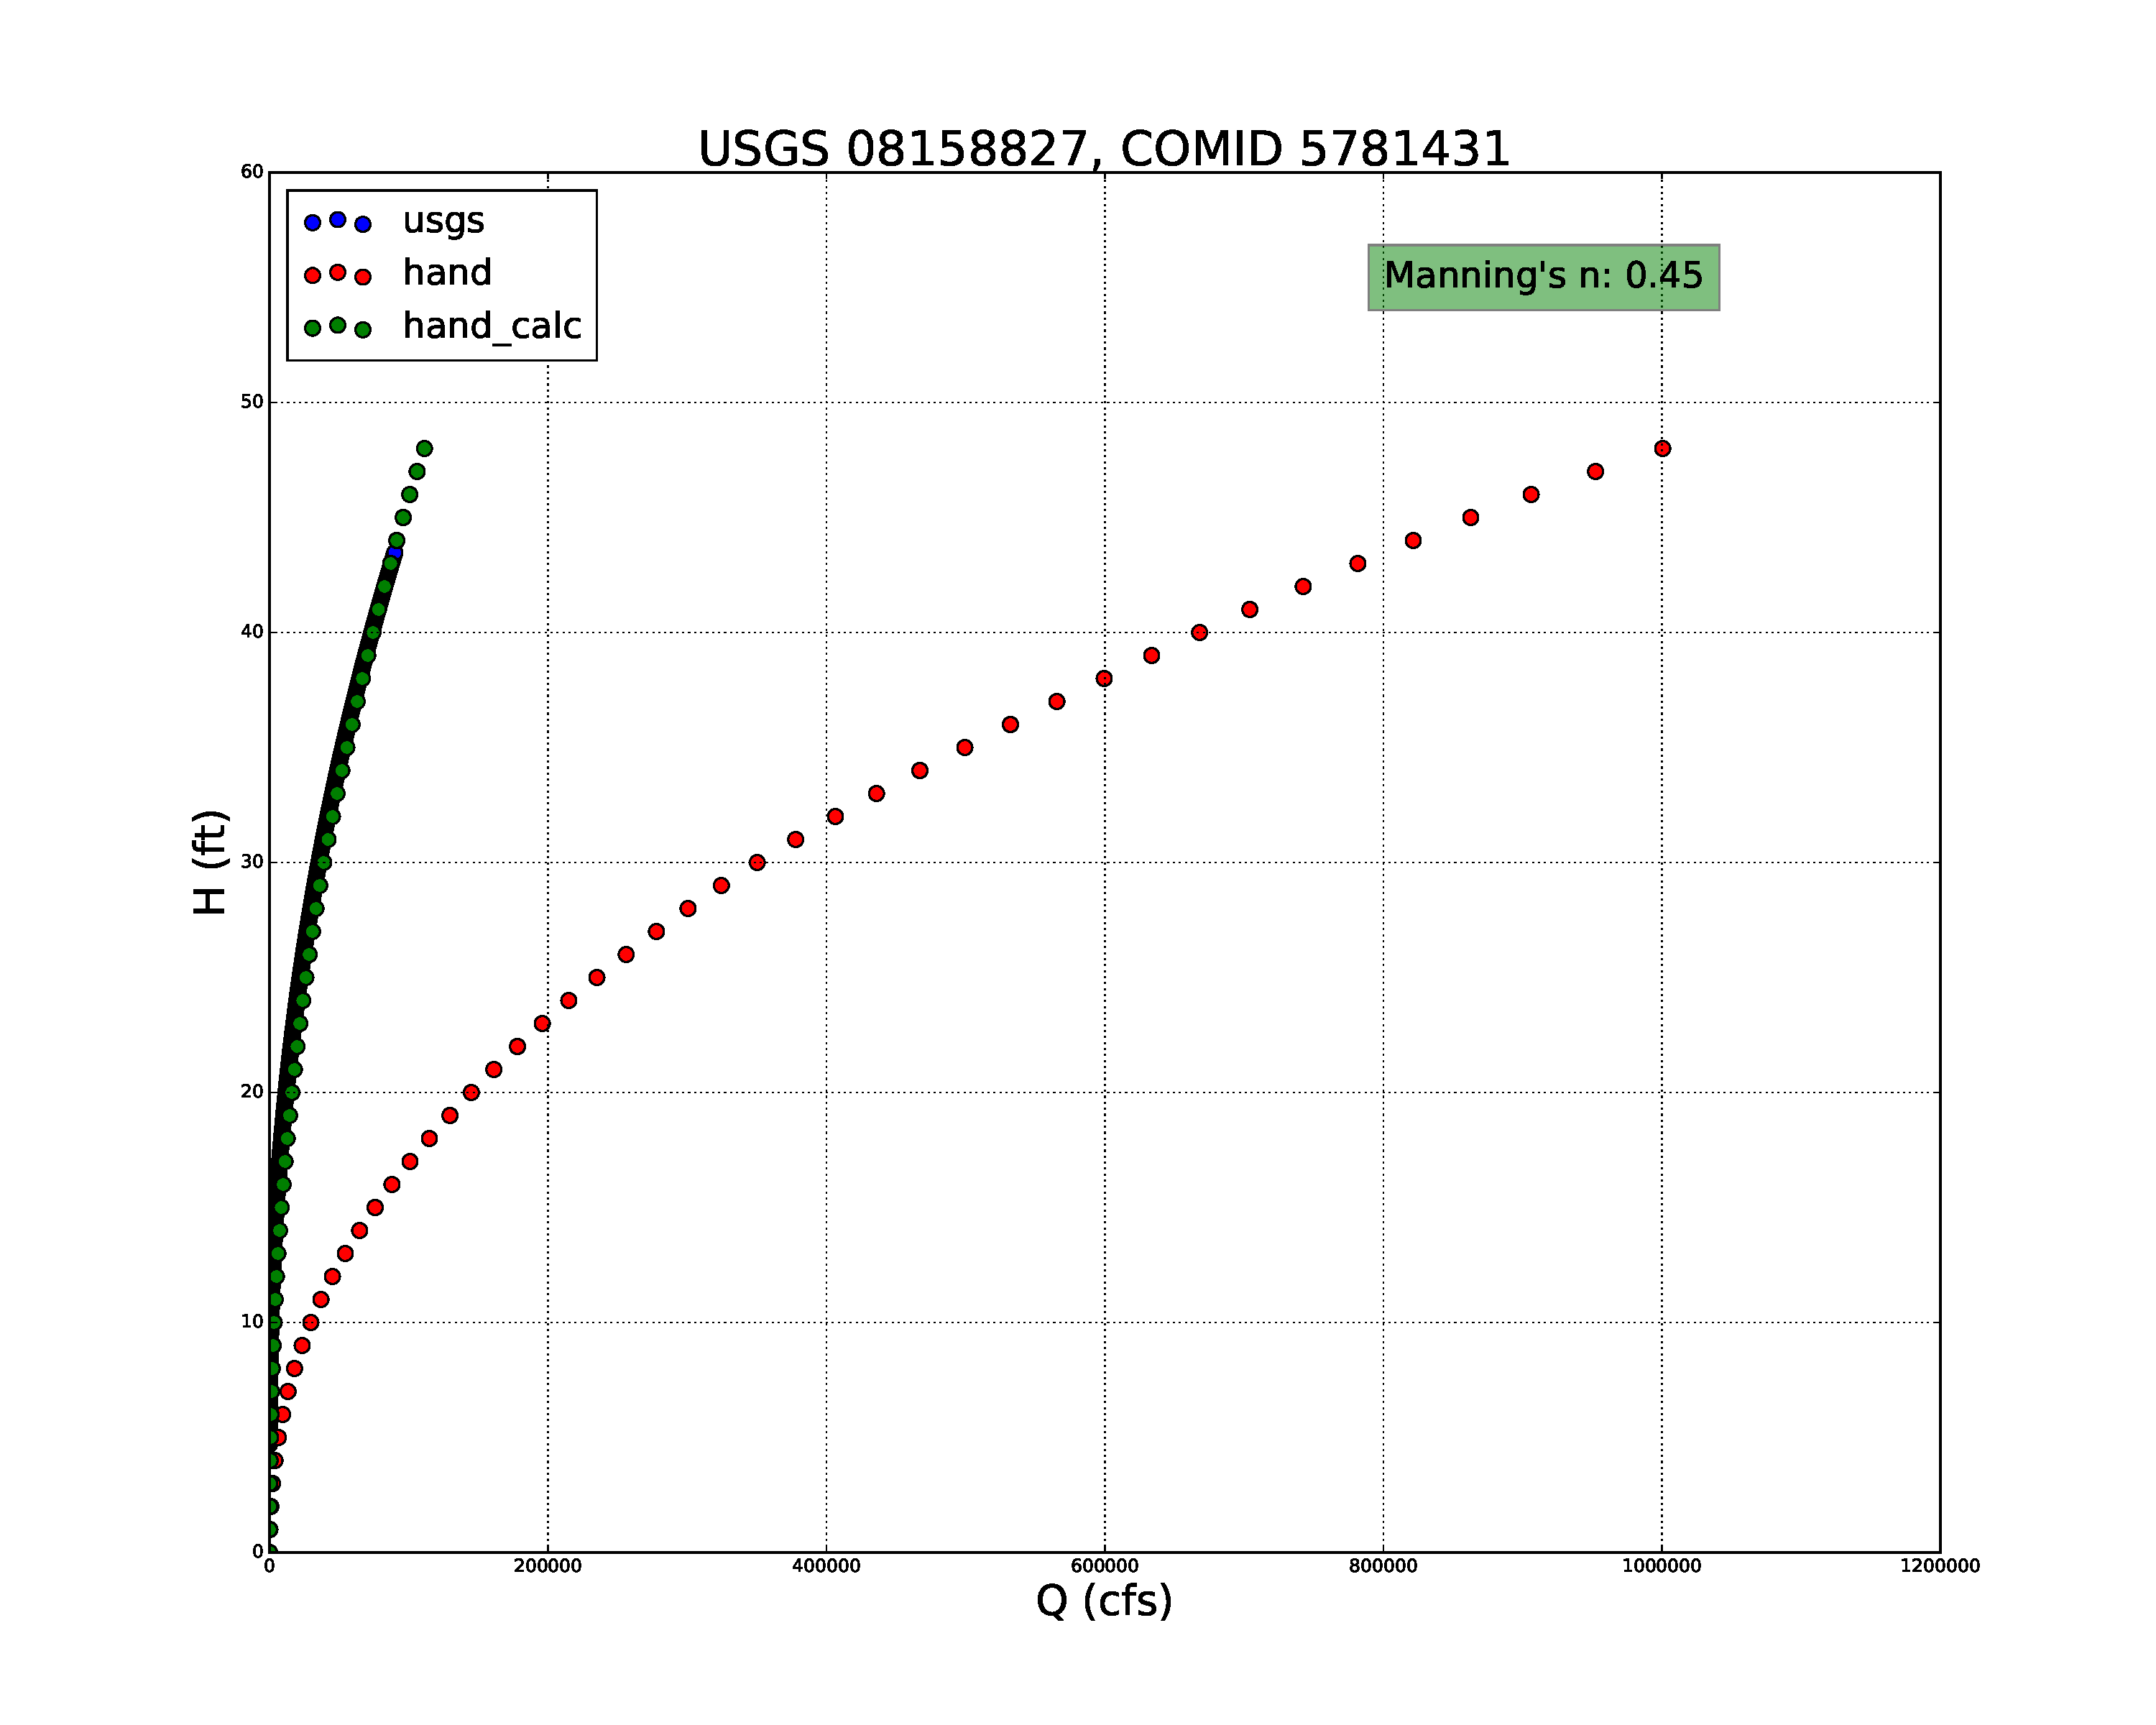
\includegraphics[width=\linewidth]{manualresults/rc_comid_5781431.pdf}
  \caption{Manually-Adjusted Rating Curve}\label{fig:a}
\end{subfigure}\hspace*{\fill}
\begin{subfigure}{0.65\textwidth}
  \centering
  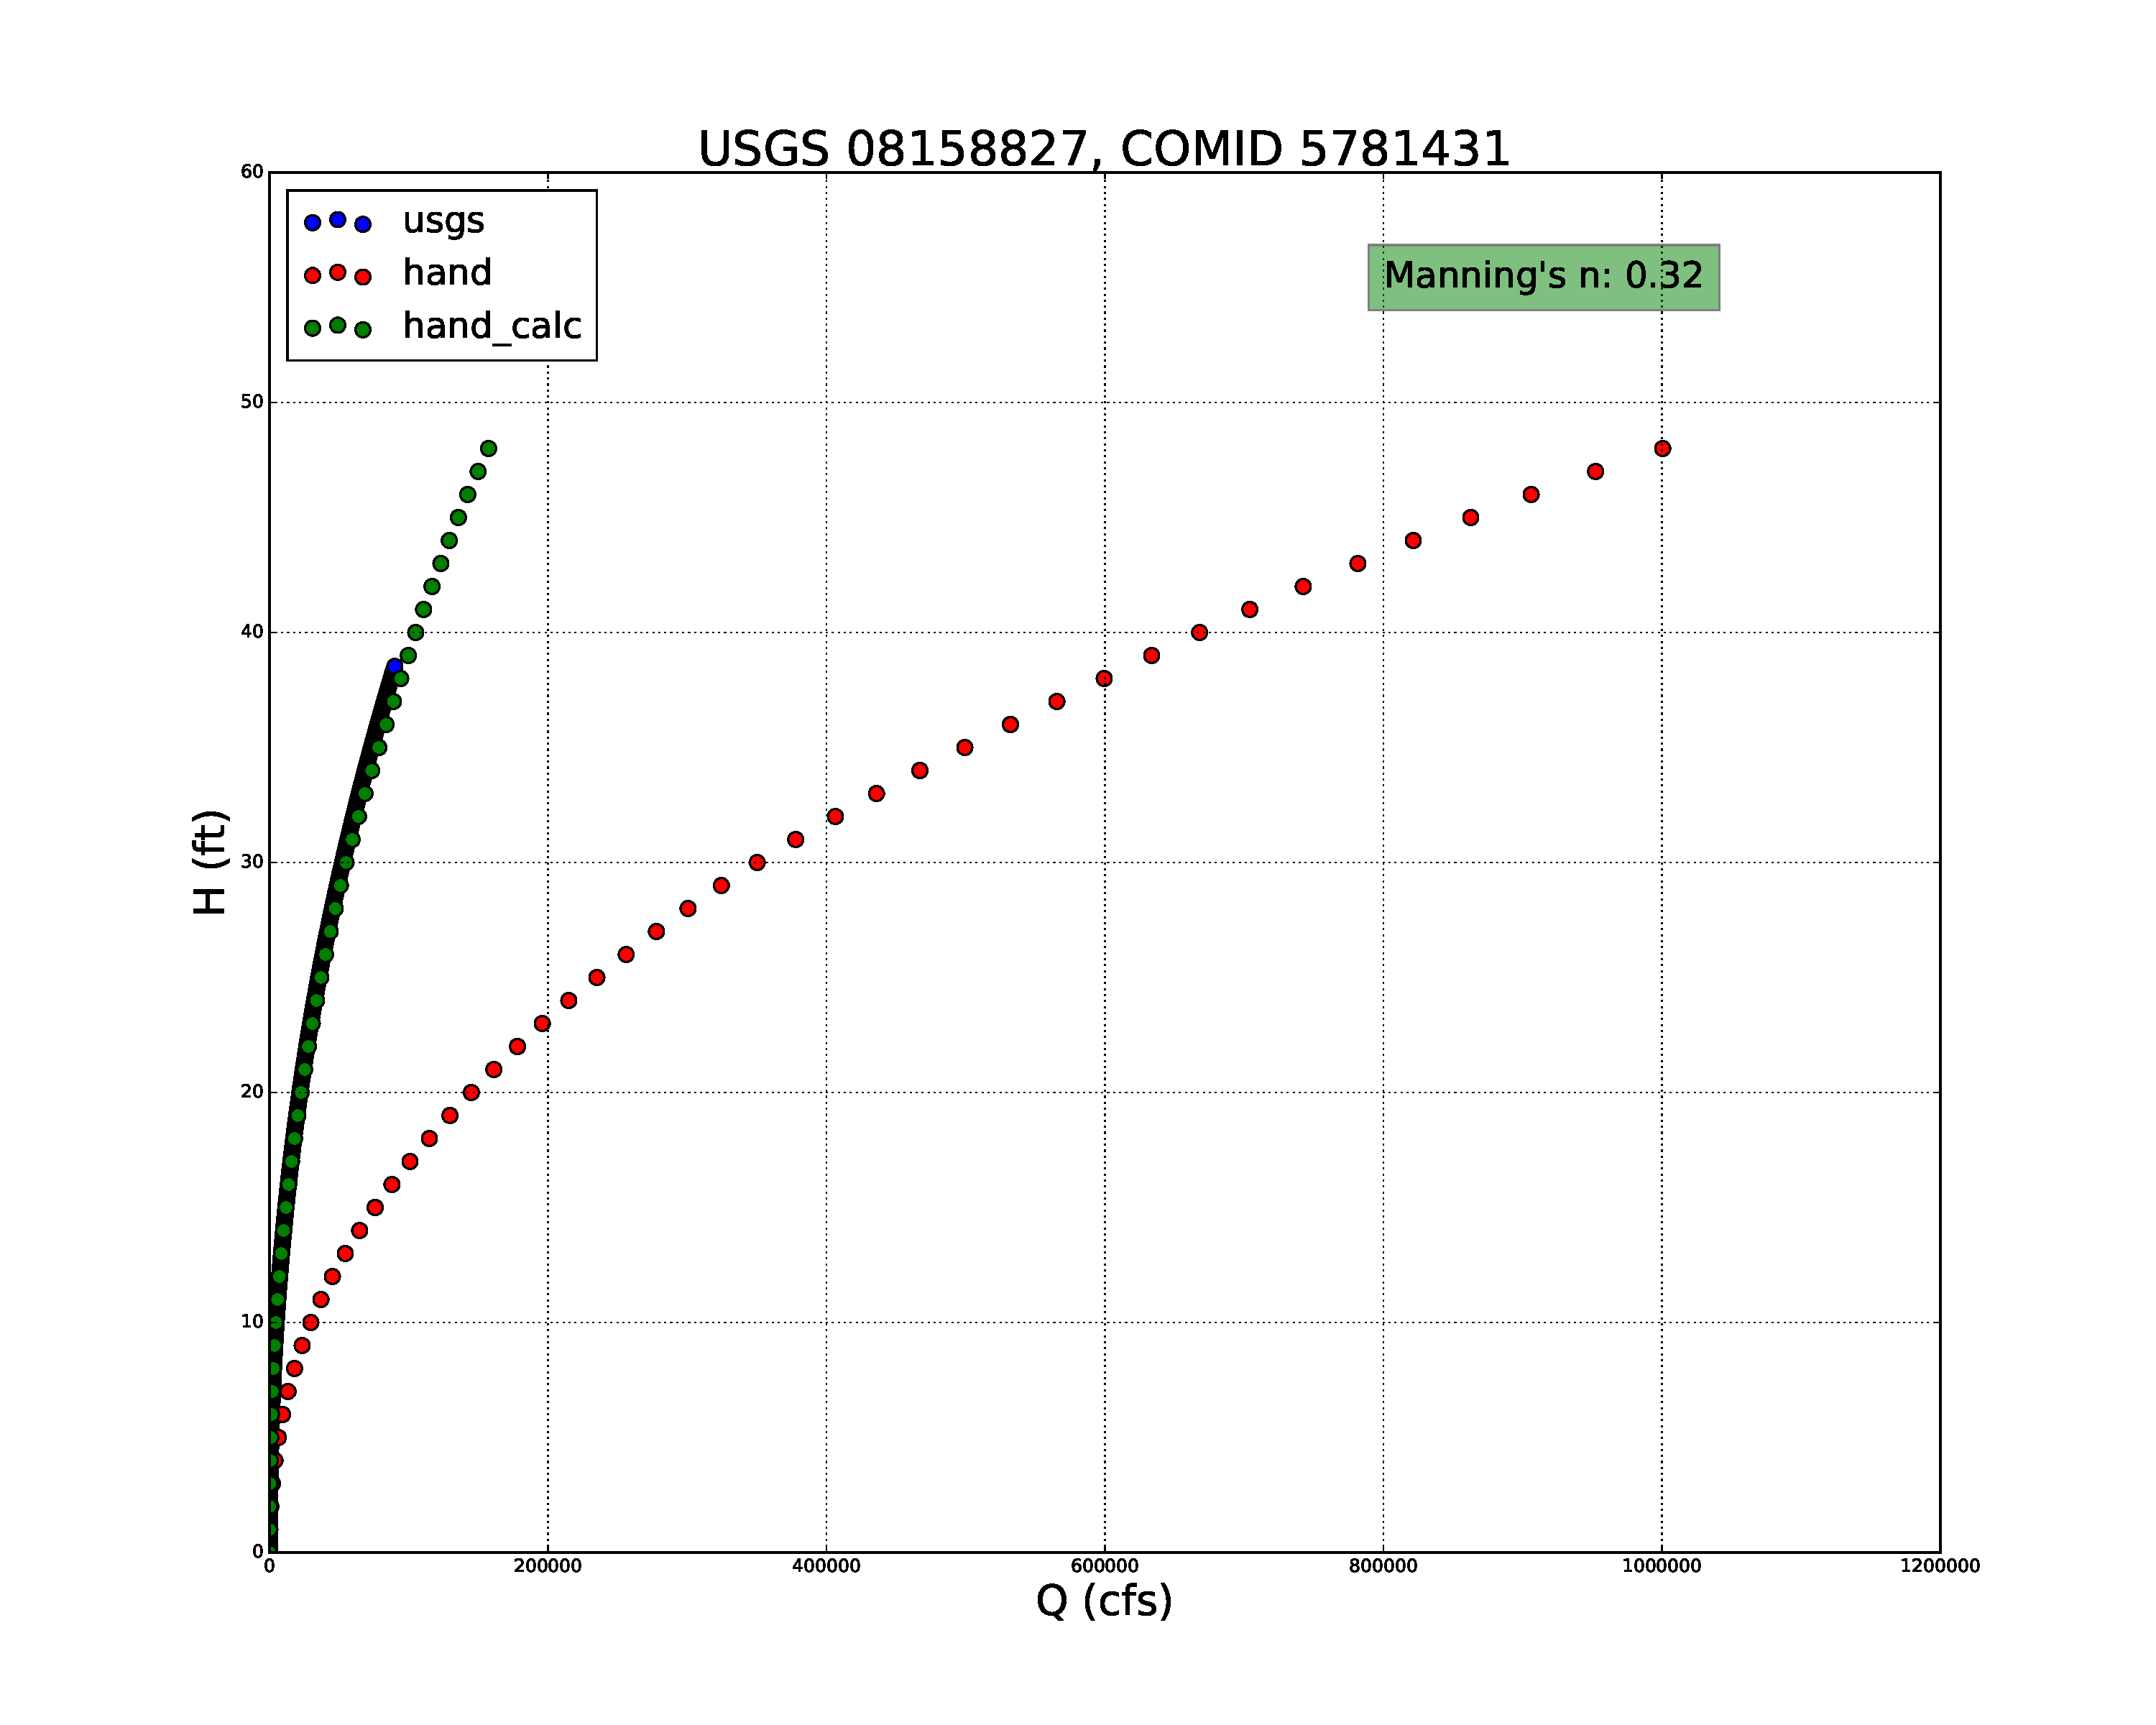
\includegraphics[width=\linewidth]{autoresults/rc_comid_5781431.pdf}
  \caption{Audomatically-Adjusted Rating Curve}\label{fig:b}
\end{subfigure}\hspace*{\fill}
}

\caption{Manual vs. Automatic Adjustments for COMID 5781431 Rating Curve} \label{fig:4}
\end{figure}

\clearpage

As stated previously, the intent of this research is to programmatically fit a HAND rating curve to its corresponding USGS rating curve. That said, manipulation of manning's $n$ is not strictly acceptable, seeing as it is a physical parameter ideally representative of the stream reach in question (see figure 4 below). Changes to manning's $n$ are effectively a claim that physical streambed material is changing, which is unreasonable. Instead, this project has changed to focus on understanding the statistical differences between "theoretical" hydrologic properties (specifically wetted area ($A_w$), hydraulic radius($H_R$), and slope ($S_0$)) and their "actual" counterparts, which will likely be retrieved from HEC-RAS models with detailed cross-section descriptions. Once these differences are understood, corrections can be approximated for each parameter that can, ideally, be used to improve the fit of each HAND rating curve. 

\begin{figure}[h]
\centering
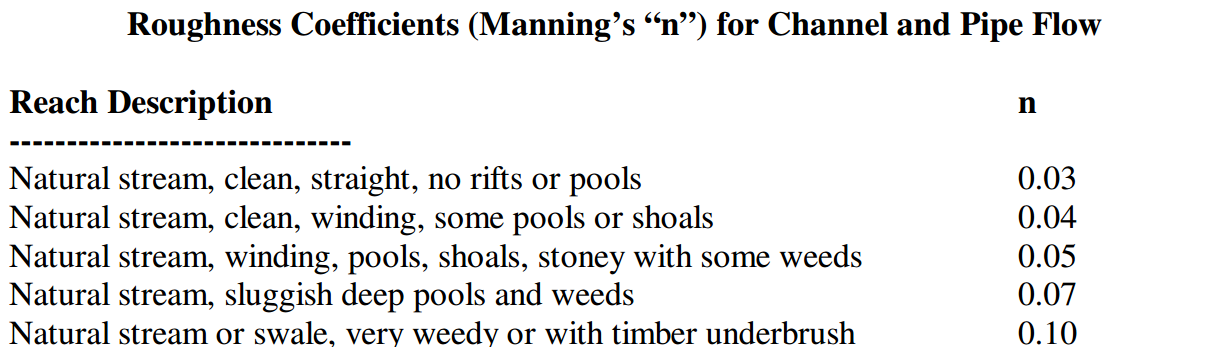
\includegraphics[keepaspectratio, width=.8\textwidth]{n_vals.png}
\caption{Acceptable Manning's $n$ values, retrieved from: \url{http://www.shippensburgtownship.com/2010-01/media/development/Table\%20B-4.pdf}} \label{fig:1}
\end{figure}

It is my current understanding that the differences between the HAND and USGS rating curves are primarily related to Digital Elevation Model (DEM) imperfections. DEMs are generally constructed with the use of remote sensing technologies, which frequently fail to penetrate through water surfaces (and, Paola, feel free to correct me if I'm wrong; you know a lot more about this than me). This failure to penetrate means that, at the time a land surface is remotely sensed, the lowest elevations for stream reaches will actually represent the stage height at that time, rather than the stream's bottom depth. Because of this discrepancy, and because HAND rasters are created from DEMs, the $A_w$ and and wetted perimeter (which together influence the $H_R$) computed from the HAND rasters may likely be incorrect (see figure 5); these discrepencies may further extend to the $S_0$, introducing another potentially faulty error to the HAND raster creation. 

\begin{figure}[t]
\centering
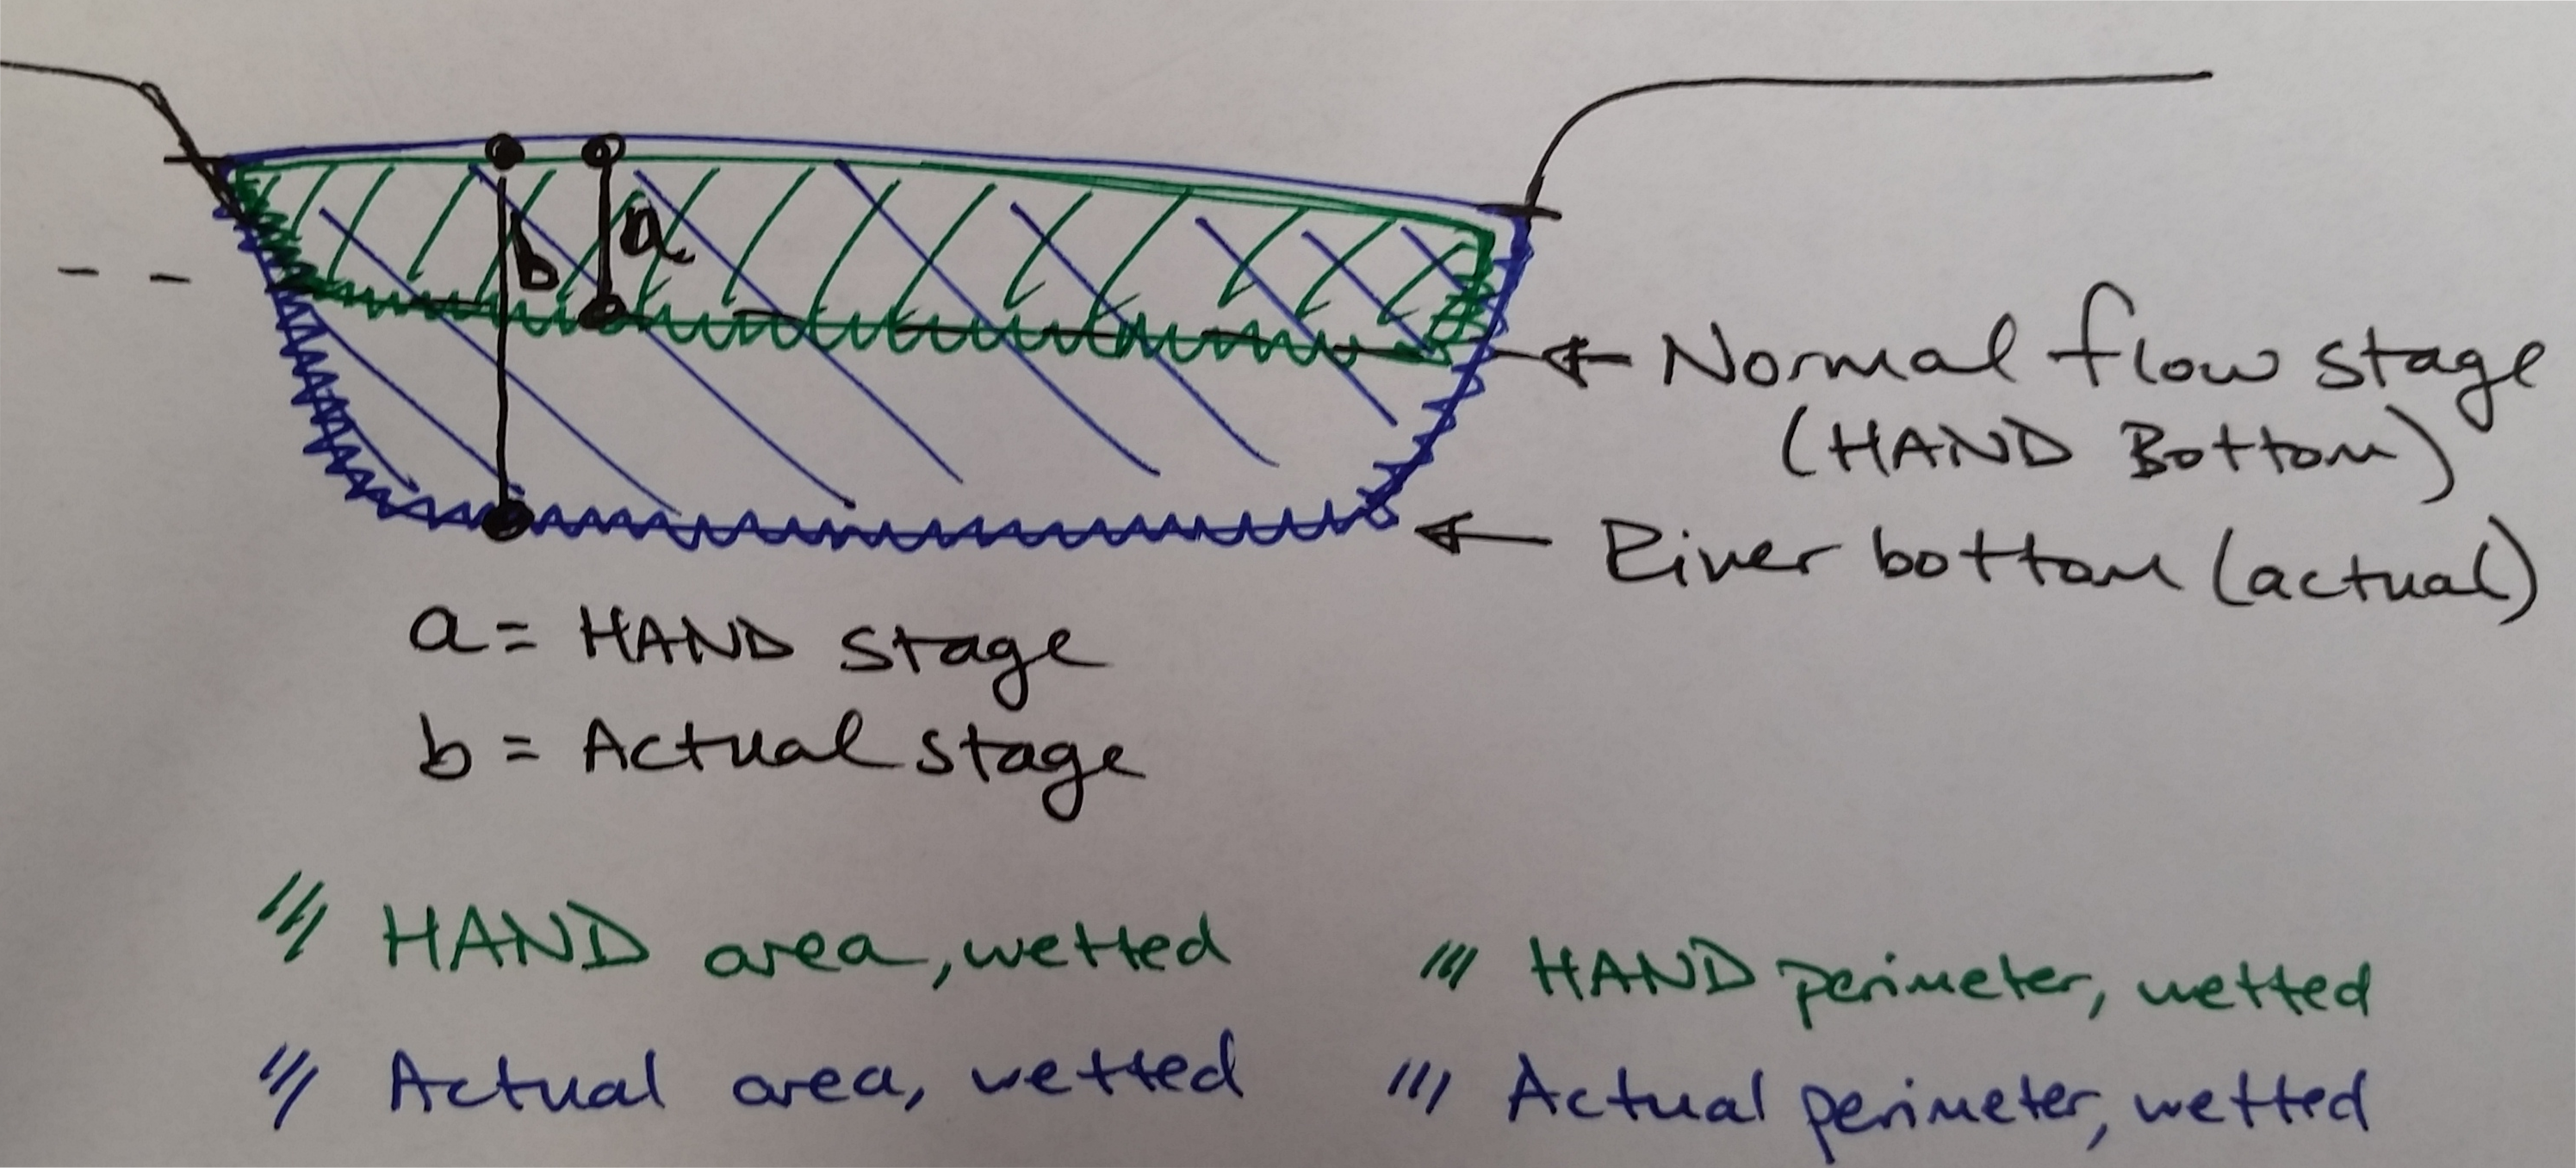
\includegraphics[keepaspectratio, width=\textwidth]{sketch.png}
\caption{Sketch of variable wetted area ($A_w$) and wetted perimeter ($P_w$)} \label{fig:5}
\end{figure}

\vspace{1ex}

No work has yet been done to access the impact of these discrepencies, but the intent of this project going forward will be to statistically analyze how different these "theoretical" (from HAND) hydraulic properties may be from their "actual" (HEC-RAS cross-sections) counterparts; note that HEC-RAS cross-section information for the Onion Creek watershed has already been retrieved (from Xing Zheng's Master's thesis work). I'm not sure yet how to approach this, but the first step will be to understand the influence of these parameters. So, for example, I will take one stream reach and gradually increase the bottom-depth shift (effectively making the HAND cross-section's bottom-depth deeper) and re-compute the resulting cross-section's $A_w$, $H_R$, and $S_0$ (this one may be a bit tricky). Once I have computed these characteristics, I will re-compute the manning's $n$ and plot the shifted HAND rating curve, comparing it to the USGS rating curve (using some form of RMSE analysis). Ultimately, I will automate this process and iterate over all possible bottom-depth shifts to arrive at the optimal bottom-depth shift. Once this optimal shift is computed for a single stream reach, I will attempt to apply my methodology to the remaining stream reaches in the Onion Creek watershed. The end goal for this approach would probably be to relate each bottom-depth shift to the average flowrate of each stream reach in some generalizable way, such that the methodology would be extendable to un-gaged stream reaches. 

If the bottom-depth shift can not be related to the average flowrate in a statistically significant manner, there may be opportunities for me to collaborate with Shahab Afshari at New York University to relate these bottom-depth shifts to the National Land Cover Dataset (NLCD). This would be a fairly complex procedure, and will likely not be completed in time for this course, but I would like very much to hear any feedback you have on that idea. Shahab is trying to relate his at-a-station hydraulic geometry computations (for approximately 5,000 USGS gage stations) to the NLCD, so we may be able to collaborate on extracting NLCD data within a buffer around each stream reach. 

\vspace{1ex}

See next page for Python script used to create curves. The major changes since the last iteration are the shift to USGS rating curves (by setting the first instance of 0.1 cfs flow as the bottom-depth) and the back-calculating of manning's $n$ values using HAND hydraulic properties ($A_w$, $H_R$, and $S_0$) and the shifted USGS rating curve. 

\clearpage

\lstinputlisting[language=Python, firstline=10, caption={Class CompareRC defined in ratingcurves-onionck.py module to quickly collect, extract, calculate, and display the USGS/HAND rating curves shown in Figures 2 through 4.}]{../../../../research/ratingcurves/ratingcurves-onionck.py}

\end{document}